\input{boilerplate}
\begin{document}
\bibliographystyle{unsrt}

\title{The encoding encyclopedia}


\author[1]{Moritz~Boos}
\author[2]{J.~Swaroop~Guntupalli}
\author[3,4]{Michael~Hanke}

\affil[1]{Oldenburg, Germany}
\affil[2]{Department of Psychological and Brain Sciences,
  Dartmouth College, Hanover, New Hampshire, USA}
\affil[3]{Psychoinformatics lab, Department of Psychology II, University of
Magdeburg, Magdeburg, Germany}
\affil[4]{Center for Behavioral Brain Sciences, Magdeburg, Germany}
\maketitle
\thispagestyle{fancy}

\listoftodos

\begin{abstract}
% Abstracts should be up to 300 words and provide a succinct summary of the
% article. Although the abstract should explain why the article might be
% interesting, care should be taken not to inappropriately over-emphasise the
% importance of the work described in the article. Citations should not be used
% in the abstract, and the use of abbreviations should be minimized.

\todo[inline]{find title}
\todo[inline]{write abstract}
\end{abstract}

\clearpage


\section*{Introduction}

\cite{CTK+2012}

\todo[inline]{any fieldstrength differences, i.e. higher resolution gives better model?}
\todo[inline]{formisano says 7T better, but more stimuli and more data with a different model are confounds}
\todo[inline]{unclear which quality metric is most appropriate due to lack of literature}
\todo[inline]{maybe add other feature sets and check metrics across all of them}

% summary: first comparative study

\todo[inline]{is this the first decode(encode(fmri)) study?}

\section*{Methods}

\cite{HBI+14,HDH+2015}

\subsection*{fMRI data}

\paragraph{\unit[3]{Tesla}}
\paragraph{\unit[7]{Tesla}}

\subsection*{Encoding model}

\todo[inline]{reference feature set description and describe encoding algorithm}

\missingfigure{encoding scheme}

\subsection*{Quality metrics}

\paragraph{Binary retrieval accuracy}

\todo[inline]{cite both mitchel and casey}

\paragraph{Correlation rank metric}

\todo[inline]{cite formisano}

\paragraph{Decoding accuracy}

%test decoding with the first PCA components of the encoded signal removed
%-->reduced accuracy by ~10%

\section*{Results}

	
%estimate size of model input (mitchel had 500, no idea why); check for 7T and 3T)
\todo[inline]{update for different nr of voxels & 3T}
\begin{figure}
	\centering
	\includegraphics[width=\linewidth]{pics/voxelnr}
	\caption{Correlation rank score as a function of the included number of voxels. The included voxels were the most stable ones i.e. their activity corresponding to each stimulus had the highest mean pairwise correlation across runs.}
	\label{fig:voxelnr}
\end{figure}
 
 
 
%binary classification accuracy result, connect to casey/mitchel
\todo[inline]{potentially other nr of voxels, take avr across all runs for 3T and 7T}
\begin{figure}
	\centering
	\includegraphics[width=\linewidth]{pics/binary_retrieval_accuracy}
	\caption{Binary retrieval classification accuracy for 3T and 7T}
	\label{fig:binretr}
\end{figure}
 
 
 
 
%correlation rankscore 3 and 7 incl. permutation analysis
\todo[inline]{potentially other nr of voxels, take avr across all runs for 3T and 7T,add permutation analysis}
\begin{figure}
	\centering
	\includegraphics[width=\linewidth]{pics/correlation_rank_score}
	\caption{Correlation rank score for 3T and 7T}
	\label{fig:rankscore}
\end{figure}
 
 
 
 
 
%decoding(encoding) accuracy: 3 vs 7 (vs. plain decoding)
\todo[inline]{potentially other nr of voxels, take avr across all runs for 3T and 7T,add discriminative classifier baseline}
\begin{figure}
	\centering
	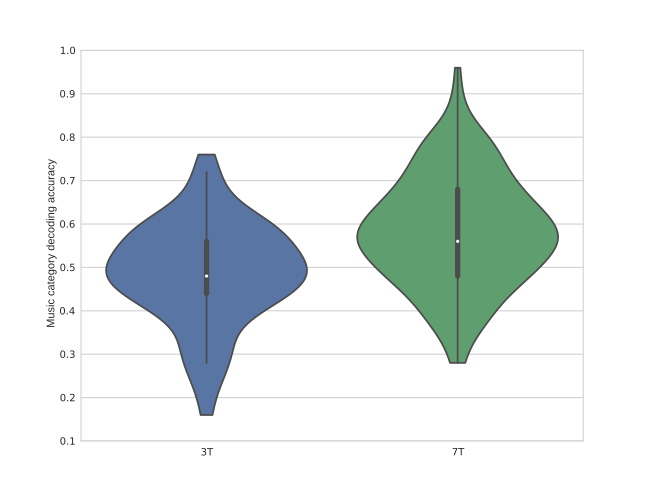
\includegraphics[width=\linewidth]{pics/decoding_accuracy}
	\caption{Decoding accuracy for 3T and 7T. A generative decoder was constructed by probabilistically inverting the encoding model.}
	\label{fig:decoder}
\end{figure}

\missingfigure{model validation on the movie}

\section*{Discussion}

\todo[inline]{7T doesnt matter -- stay cheap}

\todo[inline]{decode(encode(fmri)) vs. plain decoding}

\todo[inline]{naturalistic validation is now mandatory}


\section*{Author contributions}
%In order to give appropriate credit to each author of an article, the
%individual contributions of each author to the manuscript should be detailed
%in this section. We recommend using author initials and then stating briefly
%how they contributed.

MB performed the analysis and wrote the manuscript.
JSG contributed to the manuscript.
MH contributed to the manuscript.

\todo[inline]{describe author contributions}

\section*{Competing Interests}
No competing interests were disclosed.

\section*{Grant Information}

This research was, in part, supported by the German Federal Ministry of
Education and Research (BMBF) as part of a US-German collaboration in
computational neuroscience (CRCNS; awarded to James Haxby, Peter Ramadge, and
Michael Hanke), co-funded by the BMBF and the US National Science Foundation
(BMBF 01GQ1112; NSF 1129855).  Work on the data-sharing technology employed for
this research was supported by US-German CRCNS project awarded to
Yaroslav~O.~Halchenko and Michael~Hanke, co-funded by the BMBF and the US
National Science Foundation (BMBF 01GQ1411; NSF 1429999).  Michael Hanke was
supported by funds from the German federal state of Saxony-Anhalt, Project:
Center for Behavioral Brain Sciences.

\todo[inline]{add any financial support}

\section*{Acknowledgements}
%This section should acknowledge anyone who contributed to the research or the
%article but who does not qualify as an author based on the criteria provided
%earlier (e.g. someone or an organisation that provided writing assistance).
%Please state how they contributed; authors should obtain permission to
%acknowledge from all those mentioned in the Acknowledgements section.  Please
%do not list grant funding in this section (this should be included in the
%Grant information section - See above).

We are grateful to Michael Casey\ldots

\todo[inline]{express gratitude}

\bibliography{references}

\end{document}

% vim: textwidth=80 colorcolumn=81
